\section{Wozu Technikgeschichte?}

\subsection{Leben in einer technischen Kultur}

Die Vorlesung beginnt mit einem Gedankenexperiment: 
Man soll sich eine Gesellschaft vorstellen, die keinerlei Techniken kennt. 

Bereits nach kurzer Überlegung wird deutlich, dass eine solche Gesellschaft kaum vorstellbar ist. 
Ohne Technik gäbe es weder Elektrizität noch Fahrzeuge, keine Kommunikationsmittel, 
keine Produktionssysteme, keine Werkzeuge, keine Kleidung, keine Behausungen und 
nicht einmal symbolische Systeme wie Schrift oder Zahlen. 

Diese Überlegung führt zu einer zentralen Erkenntnis:

\begin{itemize}
    \item Technik ist kein Zusatz zur Gesellschaft.
    \item Technik ist inhärenter Bestandteil gesellschaftlichen Zusammenlebens.
    \item Technik ist Voraussetzung menschlicher Welterfahrung.
\end{itemize}

Technik ist somit nicht etwas Äusserliches oder Nachgeordnetes, sondern konstitutiv für 
menschliches Handeln, Wahrnehmen und Organisieren.

\subsection{Was ist Gegenstand der Technikgeschichte?}

Technikgeschichte beschäftigt sich nicht primär mit der Frage, 
wer eine bestimmte Maschine erfunden hat oder wie ein technisches System 
im Detail funktioniert. 

Im Zentrum steht vielmehr das Verhältnis zwischen Technik und Gesellschaft. 

Der Technikbegriff wird dabei weit gefasst. Technik umfasst:

\begin{itemize}
    \item Geräte und Maschinen
    \item Infrastrukturen
    \item Fertigkeiten und Praktiken
    \item Formen der Ausführung bestimmter Tätigkeiten
\end{itemize}

Technik ist somit nicht nur ein materielles Objekt, sondern auch eine Praxis.

\subsection{Wechselwirkungen zwischen Technik und Gesellschaft}

Technikgeschichte untersucht zwei grundlegende Fragestellungen:

\begin{enumerate}
    \item Wie verändern Techniken Gesellschaften?
    \item Wie prägen gesellschaftliche Phänomene technische Entwicklungen?
\end{enumerate}

Diese beiden Wirkungsrichtungen lassen sich meist nicht klar voneinander trennen. 
Technik beeinflusst gesellschaftliche Strukturen, während gleichzeitig soziale, 
politische und wirtschaftliche Bedingungen technische Entwicklungen formen.

Es besteht somit ein wechselseitiger Prozess, in dem Technik und Gesellschaft 
untrennbar miteinander verflochten sind.

\subsection{Fallbeispiel: Bau der Fürstenlandbrücke (1937--1941)}

\begin{center}
    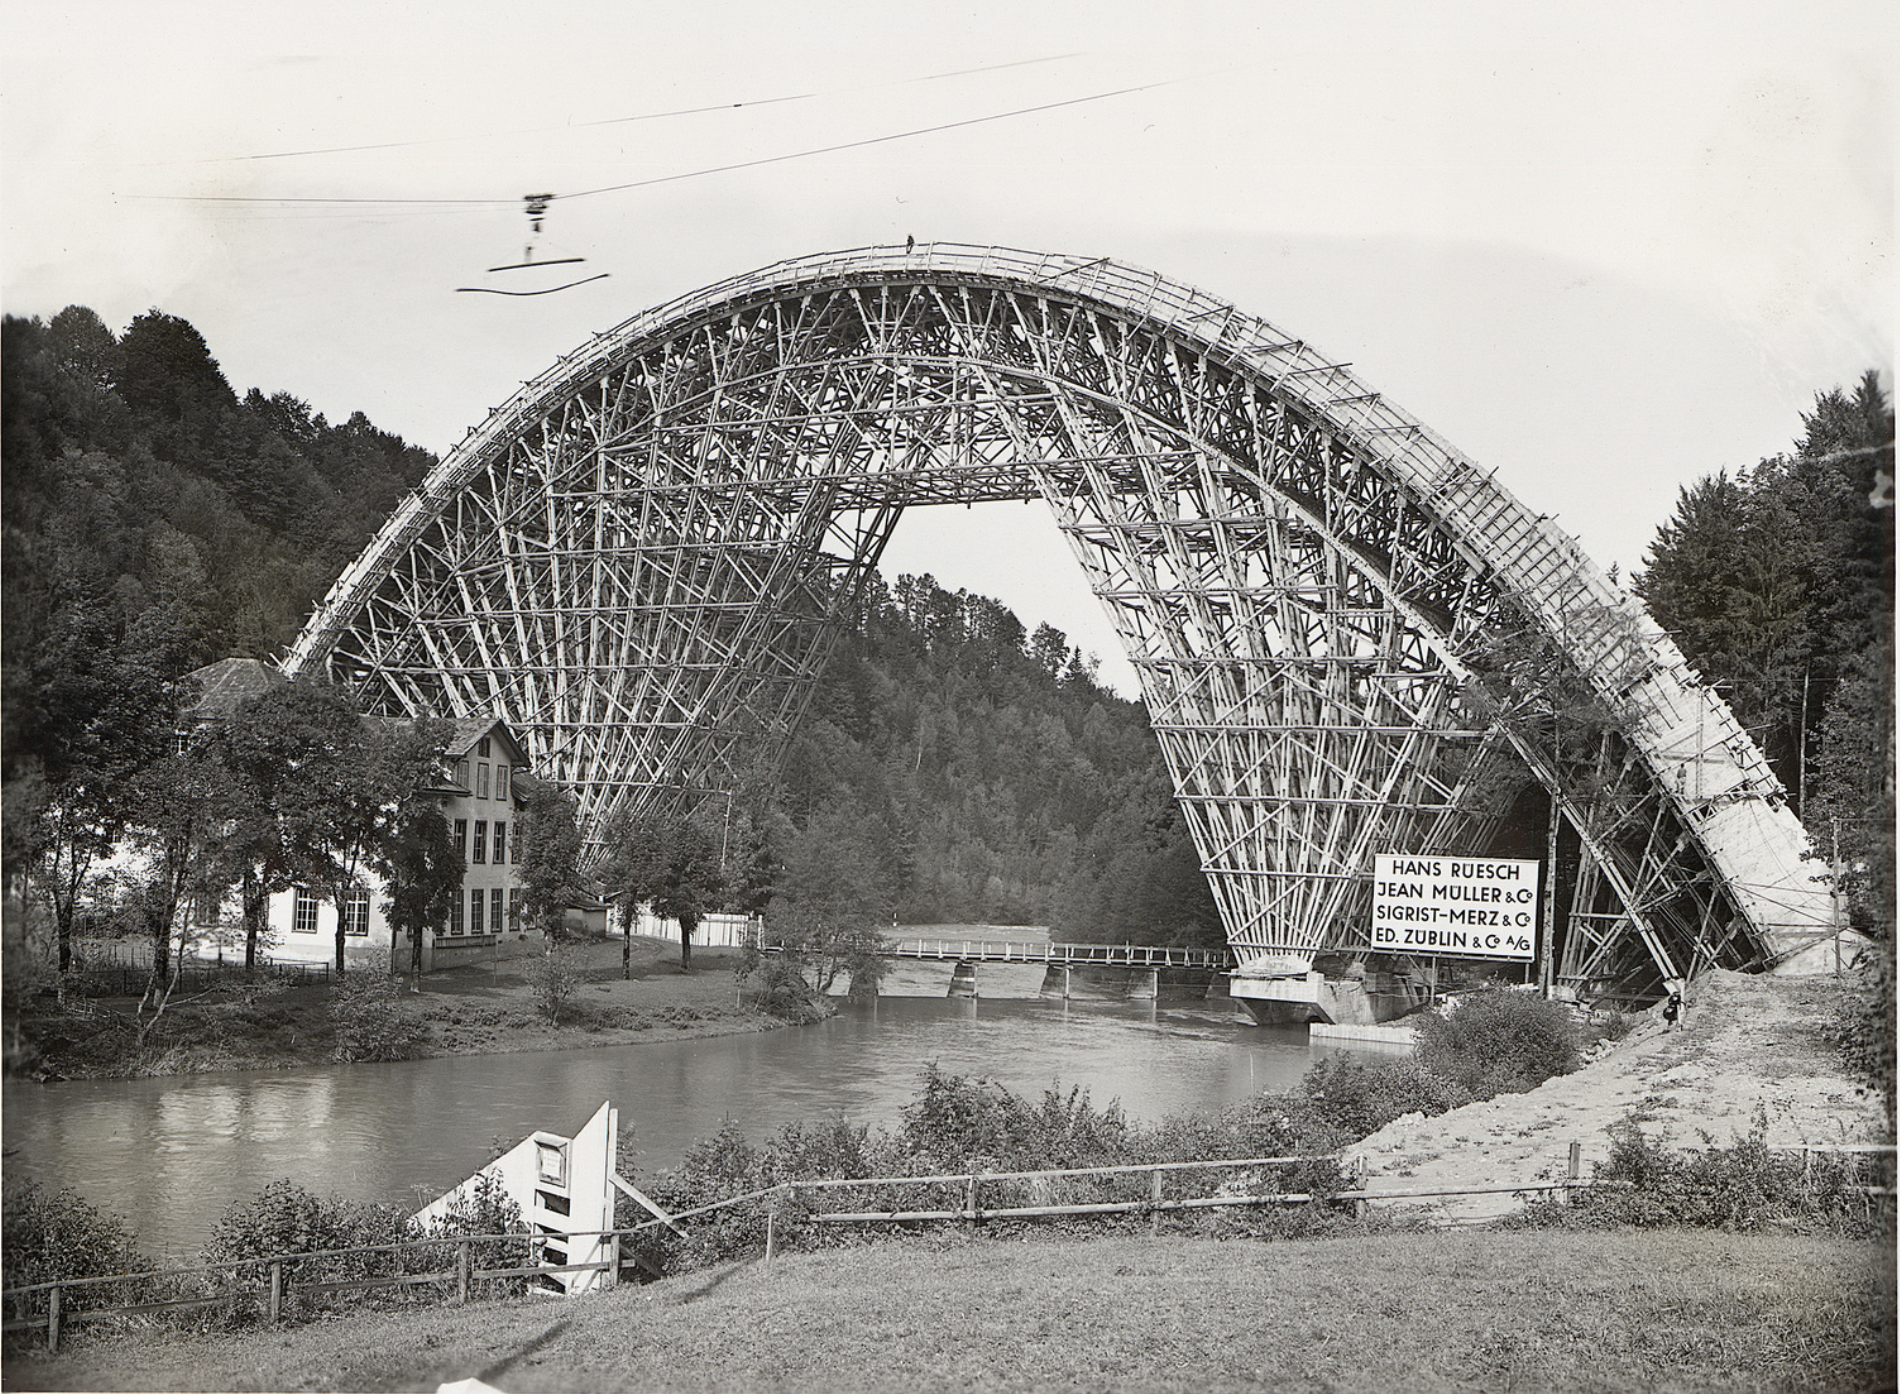
\includegraphics[width=0.8\linewidth]{images/bruecke.png}
\end{center}

Am Beispiel des Baus der Fürstenlandbrücke in St.\ Gallen wird deutlich, 
wie Technik als gesellschaftliches Phänomen analysiert werden kann.

Das Bauwerk war nicht nur eine technische Konstruktion, sondern eingebettet in 
verschiedene gesellschaftliche Kontexte:

\begin{itemize}
    \item \textbf{Mobilität:} Anpassung an neue Verkehrsmittel (Kutsche, Auto, Fahrrad, Fussverkehr).
    \item \textbf{Raumstruktur:} Verbindung von Peripherie und Zentrum durch Überwindung der Sitterschlucht.
    \item \textbf{Modernität:} Ausdruck ingenieurtechnischer Leistungsfähigkeit, Planung, Logistik und Statik.
    \item \textbf{Wirtschaft und Politik:} Arbeitsbeschaffung in einer Phase wirtschaftlicher Umbrüche.
\end{itemize}

Das Beispiel verdeutlicht, dass technische Objekte stets politische, wirtschaftliche, 
kulturelle und symbolische Dimensionen besitzen.

\subsection{Technikgeschichte als Gesellschaftsgeschichte}

Technikgeschichte arbeitet multiperspektivisch. 
Gesellschaften handeln widersprüchlich, weshalb auch technische Entwicklungen 
unterschiedlich interpretiert werden.

Wichtige Einsichten sind:

\begin{itemize}
    \item Technik determiniert ihren Nutzen oder ihre Bedeutung nicht automatisch.
    \item Technik ist nicht neutral.
    \item Akteure deuten Technik unterschiedlich.
\end{itemize}

Unterschiedliche Gruppen (Ingenieur*innen, Politiker*innen, Unternehmen, Nutzer*innen) 
verfolgen divergierende Interessen. 

Gleichzeitig besitzt Technik materielle Eigenschaften, die bestimmte Handlungen 
ermöglichen oder begrenzen. 

Technik ist somit sowohl sozial konstruiert als auch materiell wirksam.

\subsection{Methodisches Vorgehen der Geschichtswissenschaft}

Die historische Analyse beruht auf drei zentralen Elementen:

\begin{itemize}
    \item \textbf{Historische Quelle:} Bilder, Texte, Artefakte, Filme, technische Objekte.
    \item \textbf{Kontext:} Politische, ökonomische, gesellschaftliche und geopolitische Rahmenbedingungen.
    \item \textbf{Narrativ:} Perspektive und Deutung der erzählten Geschichte.
\end{itemize}

Geschichte ist somit nicht nur Rekonstruktion von Fakten, sondern immer auch 
Interpretation und Deutung.

\subsection{Ziel des Kurses}

Der Kurs verfolgt mehrere Zielsetzungen:

\begin{itemize}
    \item Sensibilisierung für die gesellschaftliche Bedeutung technischer Entscheidungen.
    \item Entwicklung historischer Urteilskompetenz.
    \item Förderung der Quellenkritik.
    \item Verständnis langfristiger technischer Entwicklungen.
\end{itemize}

Technikgeschichte soll insbesondere zukünftige Entscheidungsträger*innen 
befähigen, technische Entwicklungen nicht isoliert, sondern in ihren 
gesellschaftlichen Zusammenhängen zu reflektieren.

\subsection{Zusammenfassung}

Die zentrale Aussage der ersten Sitzung lautet:

Technik ist kein externer Faktor der Gesellschaft, sondern konstitutiver Bestandteil 
menschlicher Existenz. 

Technikgeschichte analysiert daher:

\begin{itemize}
    \item Die Wechselwirkung zwischen Technik und Gesellschaft,
    \item Die gesellschaftliche Einbettung technischer Entwicklungen,
    \item Die Deutung und Bedeutung technischer Artefakte,
    \item Die langfristigen Wirkungen technischer Entscheidungen.
\end{itemize}

Das Fach vermittelt somit nicht nur historisches Wissen, sondern 
eine reflektierte Perspektive auf die Rolle von Technik in Vergangenheit, 
Gegenwart und Zukunft.